\begin{tcolorbox}


\subsubsection*{Funções potência $f(x)=x^p$}

% \begin{enumerate}
%     \item $f(x)=x^n$, $n \in \mathrm{Z}_{+}$
%     \begin{figure}[H]
% \centering
%     \subfigure[][$n$ par]{
%     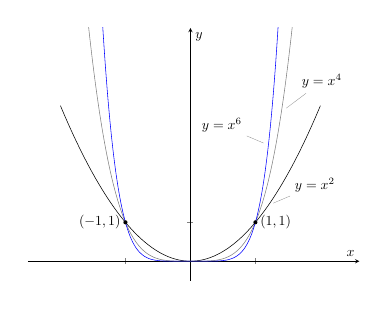
\begin{tikzpicture}[scale=0.5]
\begin{axis}[
  %title = {$f(x)=x^n$, $n=2k$, $k \in \mathrm{Z}_{+}$},
 axis lines=middle,
 ticklabel style={fill=white},
 xmin=-2.5,xmax=2.6,
 ymin=-0.5,ymax=6,
 xlabel=$x$,ylabel=$y$,
 domain=-2:2,
 samples=100,
 smooth,
 xtick={-1,0,1},ytick={1},
 yticklabels={,,},   xticklabels={,,},
 width=10cm, height=8cm]
\coordinate  (x2) at (1,1);
\coordinate (x1) at (-1,1);

\addplot[black] { x^2};
\addplot[gray] {x^4};
\addplot[blue] {x^6};
\fill[black] (x1) circle (1.5pt);
\fill[black] (x2) circle (1.5pt);

\node[pin= 20:{$y=x^2$}] at (axis cs:1.2,{(1.2)^2}) {};
\node[pin= 50:{$y=x^4$}] at (axis cs:1.4,{(1.4)^4}) {};
\node[pin= 160:{$y=x^6$}] at (axis cs:1.2,{(1.2)^6}) {};
\node[right] at (x2) {$(1,1)$};
\node[left] at (x1) {$(-1,1)$};
\end{axis}
\end{tikzpicture}














}
%     \qquad\qquad
%     \subfigure[][$n$ impar]{
%     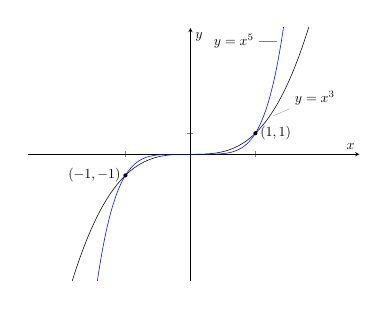
\begin{tikzpicture}[scale=0.5]
\begin{axis}[
%title = {$f(x)=x^n$, $n=2k+1$, $k \in \mathrm{Z}_{+}$},
 axis lines=middle,
 ticklabel style={fill=white},
 xmin=-2.5,xmax=2.6,
 ymin=-6,ymax=6,
 xlabel=$x$,ylabel=$y$,
 domain=-2:2,
 samples=100,
 smooth,
 xtick={-1,0,1},ytick={1},
 yticklabels={,,},   xticklabels={,,},
 width=10cm, height=8cm]
\coordinate  (x2) at (1,1);
\coordinate (x1) at (-1,-1);

\addplot[black] { x^3};
\addplot[blue] {x^5};

\fill[black] (x1) circle (1.5pt);
\fill[black] (x2) circle (1.5pt);

\node[pin= 20:{$y=x^3$}] at (axis cs:1.2,{(1.2)^3}) {};
\node[pin= 180:{$y=x^5$}] at (axis cs:1.4,{(1.4)^5}) {};

\node[right] at (x2) {$(1,1)$};
\node[left] at (x1) {$(-1,-1)$};
\end{axis}
\end{tikzpicture}}
% \end{figure}

% \item $f(x)=x^{1/n}=\sqrt[n]{x}$, $n \in \mathrm{Z}_{+}$
% \begin{figure}[H]
% \centering
%     \subfigure{
%     \begin{tikzpicture}[scale=0.5]
\begin{axis}[
 %title={$f(x)=x^{1/n}=\sqrt[n]{x}$, $n \in \mathrm{Z}_{+}$}
 axis lines=middle,
 ticklabel style={fill=white},
 xmin=-1,xmax=1.5,
 ymin=-0.5,ymax=1.5,
 xlabel=$x$,ylabel=$y$,
 domain=0:1.5,
 samples=100,
 smooth,
 xtick={-1,0,1},ytick={1},
 yticklabels={,,},   xticklabels={,,},
 width=10cm, height=6cm]
\coordinate  (x2) at (1,1);

\addplot[blue] { sqrt(x)};

\fill[black] (x2) circle (1.5pt);

\node[] at (axis cs:0.9,{(0.9)^(1/2)+0.4}) {$y=\sqrt{x}$};

\node[below right] at (x2) {$(1,1)$};

\end{axis}
\end{tikzpicture}
}
%     \qquad\qquad
%     \subfigure{
%     \begin{tikzpicture}[scale=0.5]
\begin{axis}[
 axis lines=middle,
 ticklabel style={fill=white},
 xmin=-1.5,xmax=1.5,
 ymin=-1.5,ymax=1.5,
 xlabel=$x$,ylabel=$y$,
 domain=-1.5:1.5,
 samples=100,
 smooth,
 xtick={-1,0,1},ytick={1},
 yticklabels={,,},   xticklabels={,,},
 width=10cm, height=6cm]
\coordinate  (x2) at (1,1);

\addplot[blue] {x/abs(x)*abs(x)^(1/3)};

\fill[black] (x2) circle (1.5pt);

\node[] at (axis cs:0.9,{(0.9)^(1/3)+0.4}) {$y=\sqrt[3]{x}$};
\node[below right] at (x2) {$(1,1)$};

\end{axis}
\end{tikzpicture}}
% \end{figure}

% \item $f(x)=x^{n}$, $n \in \mathrm{Z}_{-}$
% \begin{figure}[H]
%     \centering
%     \subfigure{
%     \begin{tikzpicture}[scale=0.5]
\begin{axis}[
 axis lines=middle,
 ticklabel style={fill=white},
 xmin=-1.5,xmax=1.5,
 ymin=-4,ymax=4,
 xlabel=$x$,ylabel=$y$,
 domain=-1.5:1.5,
 samples=100,
 smooth,
 xtick={-1,0,1},ytick={1,-1},
 yticklabels={,,},   xticklabels={,,},
 width=10cm]
\coordinate  (x2) at (1,1);
\coordinate  (x1) at (-1,-1);
\addplot[blue] {1/x};


\fill[black] (x2) circle (1.5pt);
\fill[black] (x1) circle (1.5pt);

\node[] at (axis cs:0.8,{1/(0.8)+1}) {$y=\dfrac{1}{x}$};

\node[above right] at (x2) {$(1,1)$};
\node[above right] at (x1) {$(-1,-1)$};

\end{axis}
\end{tikzpicture}}
%     \qquad\qquad
%     \subfigure{
% \begin{tikzpicture}[scale=0.5]
\begin{axis}[
 axis lines=middle,
 ticklabel style={fill=white},
 xmin=-1.5,xmax=1.5,
 ymin=-1,ymax=5,
 xlabel=$x$,ylabel=$y$,
 domain=-1.4:1.4,
 samples=30,
 smooth,
 xtick={-1,0,1},ytick={1},
 yticklabels={,,},   xticklabels={,,},
 width=10cm]
\coordinate  (x2) at (1,1);
\coordinate  (x1) at (-1,1);
\addplot[blue] {1/x^2};


\fill[black] (x2) circle (1.5pt);
\fill[black] (x1) circle (1.5pt);

\node[] at (axis cs:0.9,{1/(0.8)^2+1.5}) {$y=\dfrac{1}{x^2}$};


\node[above right] at (x2) {$(1,1)$};
\node[above left] at (x1) {$(-1,1)$};
\end{axis}
\end{tikzpicture}}
% \end{figure}

% \end{enumerate}

\begin{figure}[H]
\centering
    \subfigure{
    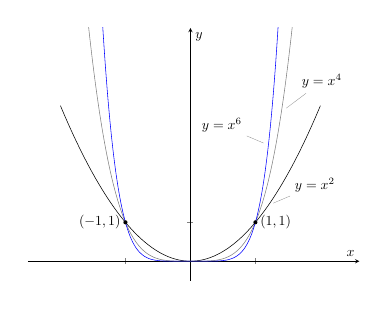
\begin{tikzpicture}[scale=0.5]
\begin{axis}[
  %title = {$f(x)=x^n$, $n=2k$, $k \in \mathrm{Z}_{+}$},
 axis lines=middle,
 ticklabel style={fill=white},
 xmin=-2.5,xmax=2.6,
 ymin=-0.5,ymax=6,
 xlabel=$x$,ylabel=$y$,
 domain=-2:2,
 samples=100,
 smooth,
 xtick={-1,0,1},ytick={1},
 yticklabels={,,},   xticklabels={,,},
 width=10cm, height=8cm]
\coordinate  (x2) at (1,1);
\coordinate (x1) at (-1,1);

\addplot[black] { x^2};
\addplot[gray] {x^4};
\addplot[blue] {x^6};
\fill[black] (x1) circle (1.5pt);
\fill[black] (x2) circle (1.5pt);

\node[pin= 20:{$y=x^2$}] at (axis cs:1.2,{(1.2)^2}) {};
\node[pin= 50:{$y=x^4$}] at (axis cs:1.4,{(1.4)^4}) {};
\node[pin= 160:{$y=x^6$}] at (axis cs:1.2,{(1.2)^6}) {};
\node[right] at (x2) {$(1,1)$};
\node[left] at (x1) {$(-1,1)$};
\end{axis}
\end{tikzpicture}














}
    \qquad
    \subfigure{
    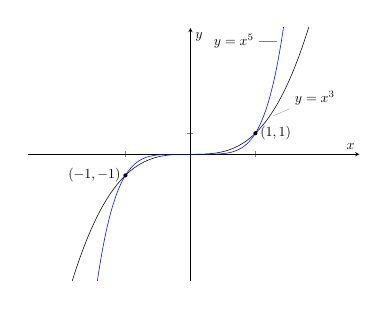
\begin{tikzpicture}[scale=0.5]
\begin{axis}[
%title = {$f(x)=x^n$, $n=2k+1$, $k \in \mathrm{Z}_{+}$},
 axis lines=middle,
 ticklabel style={fill=white},
 xmin=-2.5,xmax=2.6,
 ymin=-6,ymax=6,
 xlabel=$x$,ylabel=$y$,
 domain=-2:2,
 samples=100,
 smooth,
 xtick={-1,0,1},ytick={1},
 yticklabels={,,},   xticklabels={,,},
 width=10cm, height=8cm]
\coordinate  (x2) at (1,1);
\coordinate (x1) at (-1,-1);

\addplot[black] { x^3};
\addplot[blue] {x^5};

\fill[black] (x1) circle (1.5pt);
\fill[black] (x2) circle (1.5pt);

\node[pin= 20:{$y=x^3$}] at (axis cs:1.2,{(1.2)^3}) {};
\node[pin= 180:{$y=x^5$}] at (axis cs:1.4,{(1.4)^5}) {};

\node[right] at (x2) {$(1,1)$};
\node[left] at (x1) {$(-1,-1)$};
\end{axis}
\end{tikzpicture}}
    \subfigure{
    \begin{tikzpicture}[scale=0.5]
\begin{axis}[
 %title={$f(x)=x^{1/n}=\sqrt[n]{x}$, $n \in \mathrm{Z}_{+}$}
 axis lines=middle,
 ticklabel style={fill=white},
 xmin=-1,xmax=1.5,
 ymin=-0.5,ymax=1.5,
 xlabel=$x$,ylabel=$y$,
 domain=0:1.5,
 samples=100,
 smooth,
 xtick={-1,0,1},ytick={1},
 yticklabels={,,},   xticklabels={,,},
 width=10cm, height=6cm]
\coordinate  (x2) at (1,1);

\addplot[blue] { sqrt(x)};

\fill[black] (x2) circle (1.5pt);

\node[] at (axis cs:0.9,{(0.9)^(1/2)+0.4}) {$y=\sqrt{x}$};

\node[below right] at (x2) {$(1,1)$};

\end{axis}
\end{tikzpicture}
}
    \qquad
    \subfigure{
    \begin{tikzpicture}[scale=0.5]
\begin{axis}[
 axis lines=middle,
 ticklabel style={fill=white},
 xmin=-1.5,xmax=1.5,
 ymin=-1.5,ymax=1.5,
 xlabel=$x$,ylabel=$y$,
 domain=-1.5:1.5,
 samples=100,
 smooth,
 xtick={-1,0,1},ytick={1},
 yticklabels={,,},   xticklabels={,,},
 width=10cm, height=6cm]
\coordinate  (x2) at (1,1);

\addplot[blue] {x/abs(x)*abs(x)^(1/3)};

\fill[black] (x2) circle (1.5pt);

\node[] at (axis cs:0.9,{(0.9)^(1/3)+0.4}) {$y=\sqrt[3]{x}$};
\node[below right] at (x2) {$(1,1)$};

\end{axis}
\end{tikzpicture}}
    \subfigure{
    \begin{tikzpicture}[scale=0.5]
\begin{axis}[
 axis lines=middle,
 ticklabel style={fill=white},
 xmin=-1.5,xmax=1.5,
 ymin=-4,ymax=4,
 xlabel=$x$,ylabel=$y$,
 domain=-1.5:1.5,
 samples=100,
 smooth,
 xtick={-1,0,1},ytick={1,-1},
 yticklabels={,,},   xticklabels={,,},
 width=10cm]
\coordinate  (x2) at (1,1);
\coordinate  (x1) at (-1,-1);
\addplot[blue] {1/x};


\fill[black] (x2) circle (1.5pt);
\fill[black] (x1) circle (1.5pt);

\node[] at (axis cs:0.8,{1/(0.8)+1}) {$y=\dfrac{1}{x}$};

\node[above right] at (x2) {$(1,1)$};
\node[above right] at (x1) {$(-1,-1)$};

\end{axis}
\end{tikzpicture}}
    \qquad\qquad
    \subfigure{
\begin{tikzpicture}[scale=0.5]
\begin{axis}[
 axis lines=middle,
 ticklabel style={fill=white},
 xmin=-1.5,xmax=1.5,
 ymin=-1,ymax=5,
 xlabel=$x$,ylabel=$y$,
 domain=-1.4:1.4,
 samples=30,
 smooth,
 xtick={-1,0,1},ytick={1},
 yticklabels={,,},   xticklabels={,,},
 width=10cm]
\coordinate  (x2) at (1,1);
\coordinate  (x1) at (-1,1);
\addplot[blue] {1/x^2};


\fill[black] (x2) circle (1.5pt);
\fill[black] (x1) circle (1.5pt);

\node[] at (axis cs:0.9,{1/(0.8)^2+1.5}) {$y=\dfrac{1}{x^2}$};


\node[above right] at (x2) {$(1,1)$};
\node[above left] at (x1) {$(-1,1)$};
\end{axis}
\end{tikzpicture}}
\end{figure}
\end{tcolorbox}
% \subsubsection*{Função Módulo}
% Seja $x,y \in \mathbb{R}$ então:
% \begin{align*}
%     |x|=\begin{cases}
%      x \quad \text{se} \quad x\leq 0  \\
%      -x\quad \text{se} \quad x< 0
%     \end{cases}
% \end{align*}

% \begin{multicols}{2}
% \subsubsection*{Propriedades}
% $|xy|=|x||y|$\\
% $\left|\dfrac{x}{y}\right|=\dfrac{|x|}{|y|}$\\
% $|x^n|=|x|^n$\\
% $\sqrt{x^2}=|x|$\\
% $|x+y|\leq |x|+|y|$ \qquad (desigualdade triangular)
% \columnbreak
% \subsubsection*{Gráfico}
% \begin{Figure}
%     \begin{tikzpicture}[scale=0.5]
\begin{axis}[
 axis lines=middle,
 ticklabel style={fill=white},
 xmin=-1.5,xmax=1.5,
 ymin=-0.5,ymax=1.5,
 xlabel=$x$,ylabel=$y$,
 domain=-1.2:1.2,
 samples=100,
 smooth,
 xtick={-1,0,1},ytick={1},
 yticklabels={,,},   xticklabels={,,},
 width=10cm]
\coordinate  (x2) at (1,1);
\coordinate  (x1) at (-1,-1);
\addplot[blue] {abs(x)};

\node[] at (axis cs:0.8,1.2) {$y=|x|$};
\end{axis}
\end{tikzpicture}
% \end{Figure}
% \end{multicols}

